\chapter{Research}
\section{Version history}
\begin{table}[H]
\begin{tabular}{|c|p{9cm}|c|c|}
\hline
Version & Description & Author & Date\\
\hline
0.1 & Initial draft & JK & 29/12-13\\
\hline
0.2 & Updated Parotec description & NG & 09/01-14\\
\hline
\end{tabular}
\end{table}

\section{Purpose}
The purpose of this document is to present all technologies, literature and prior art related to the project. This document should be updated and versioned during the project to make sure all references and documentation is listed.

\section{References}
$\bullet$ Project description

\section{Glossary}
\begin{table}[H]
\centering
\begin{tabular}{|p{4cm}|p{7cm}|}
\hline
Term & Definition\\ \hline
&\\ \hline
\end{tabular}
\end{table}

\section{Literature}

%Brugt som guideline til referencer http://www.lc.unsw.edu.au/onlib/pdf/elect_ref.pdf

\begin{table}[H]
\centering
\begin{tabular}{|p{4cm}|p{10cm}|}
\hline
Description & Reference\\ \hline
Medical note on feet temperature&Nardin RA, Rogerson PM, Nie R, Rutkove SB, 'Foot temperature in healthy individuals: effects of ambient temperature and age.', \textit{Journal of the American Podiatric Medical Association}, accessed 17 December 2013, <\url{http://www.ncbi.nlm.nih.gov/pubmed/20660876}>\\ \hline
& \\ \hline
\end{tabular}
\end{table}

\section{Prior art}
Below is a list of similar prior art. A quick comparison of the product and project will be explained.
\subsection{ShoePad Diabetic $^{TM}$}
\textbf{Patent:} WO/2009/005373A1
\subsubsection{Description}
\begin{wrapfigure}{r}{5cm}
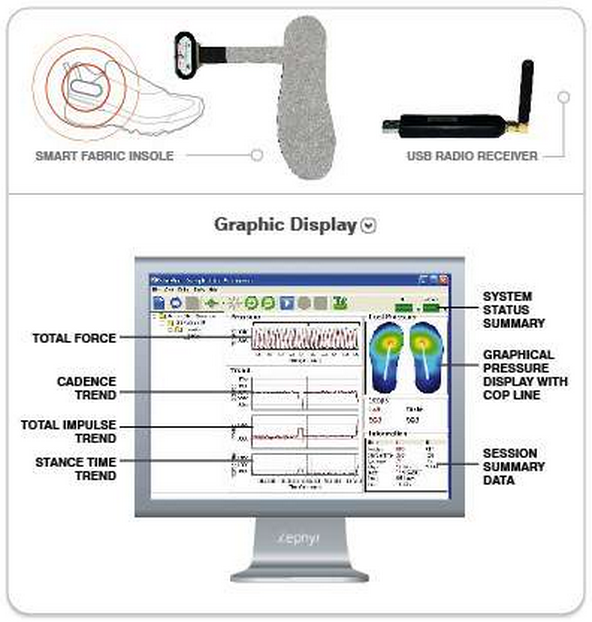
\includegraphics[width=5cm]{billeder/shoepad}
\caption{Figure describing the Shoepad}
\end{wrapfigure}
The system comprises of an insole which has a number of temperature sensors. Theses insoles has a radio transmitter which connects to a computer or watch. The system compares the temperature of both feed and can give an audible or visual alarm if the temperature difference is at a critical level.
\subsubsection{Similarities}
This system will in many ways be very similar to that of the group since the purpose is exactly the same. This system has a number of temperature sensors and the system can based on the values indicate an alarm to the user.
\subsubsection{Differences}
This system is only in the insole and therefore the temperature is only monitored on the bottom of the feet.\\
This system transmits the data via. radio signal and must therefore be within range of the computer which it is connected to. This limits what the user are able to do while wearing the insole.

\subsection{TempTablet}
\textbf{Patent:} none found.
\subsubsection{Description}
\begin{wrapfigure}{r}{5cm}
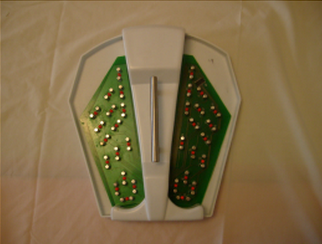
\includegraphics[width=5cm]{billeder/temptablet}
\caption{Image of the TempTablet}
\end{wrapfigure}
The system has a scale/weight-like formfactor and is meant to be used by patients daily. It can store data locally on an SD-card. But it also has some wireless connections although nothing of their use is mentioned in the article.
\subsubsection{Similarities}
The system is meant to be used by patients and monitoring the feet temperature. It can give an alarm depending on the values of these data.
\subsubsection{Differences}
The system is not very mobile because of the formfactor. Therefore it cannot constantly monitor the feet.\\


\subsection{Parotec}
\textbf{Patent:} US5642096
\subsubsection{Description}
The system is based around a shoe/insole solution. The insole is has hydrocell pressure and temperature sensors. A controller with an elastic strap for mounting on the stomach is used. The controller has an alarm function.
\subsubsection{Similarities}
The system features a central data unit that collection measurements from the sensors. The data can be transferred to a tool on computer. Based on profiles, the system can warn the user about issues with pressure. 
\subsubsection{Differences}
The sensors are placed in a sole and concentrated around the front of the foot. The system measures pressure. Although mentioned in the patent the system does not measure temperature.
%\begin{table}[H]
%\begin{tabular}{|p{4cm}|p{3.5cm}|p{7cm}|}
%\hline
%Product & Patent & description\\ \hline
%ShoePod Diabetic$^{TM}$ & WO/2009/005373A1 & Shoe/insole. Smart fabric technology. Pressure and temperature sensor arrays. Chip thermistors. \\ \hline
%TempTablet & none & Sensor arrays. Temperature profiles of the feet. Storage of data for comparisons. Alarm function. \\ \hline
%Parotec & US5642096 & Shoe/insole. Hydrocell pressure and temperature sensors. Alarm function. \\ \hline
%\end{tabular}
%\end{table}
%Lignenede devices: \url{http://www.diva-portal.org/smash/get/diva2:359794/FULLTEXT01.pdf} side 17\\